
\section{Finding Multiple Objects}

\todo[inline, color=red!50]{Add topic: Viola Jones (face detection)}

The problem at the core is how to scan many positions efficiently for possible faces. Possible approaches are
\begin{itemize}[label=-, nosep]
	\item {\color{DodgerBlue4} Features}
	\item {\color{DodgerBlue4} Classifier}
	\item {\color{DodgerBlue4} Sliding Window}
	\item {\color{Firebrick1} Haar Features}
	\item {\color{Firebrick1} Boosting}
	\item {\color{Firebrick1} Cascaded Classifiers}
\end{itemize}

\subsection{Boosting}
For an input training data with weights, at each step $t \in 1..T$ train a weak classifier,
let it classify the training data and increase the weight on incorrectly classified samples.
Use the weighted combination of all weak classifiers for the final, strong classifier.
The final strong classifier $F(x)$ can be understood as a weighted, linear combination of the weak classifiers.
\begin{equation*}
	F(x) = \alpha_1 f_1(x) + \alpha_2 f_2(x) + \alpha_2 f_2(x) + \dots
\end{equation*}
Weak classifier used with $f$ feature, $\theta$ threshold and $p_j$ parity
\begin{equation*}
	h_j (\theta) = \left\{ \begin{matrix}
		1 & p_j f_j < p_j \theta_j\\
		0 & \text{otherwise}
		\end{matrix} \right.
\end{equation*}

\subsection{Haar Features}
Filter responses, that is convolutions, are computationally intensive. The idea of haar features is to only use
simple filters of different sizes and shapes with only $-1$ or $1$ in the masks.
Calculate the features on sliding sub windows (for example $24\times24$ pixels) and take all possible combinations of
filters as feature candidates. This can be done in a fast manner using integral images,
where each pixel of the integral image contains the sum of all values in the
rectangle spanned to the upper left corner (see image \ref{fig:integralimage}).
The sum of pixel $D$ in figure \ref{fig:integralimagehaar} is $4 + 1 - (2 + 3)$ or in terms of the named rectangles
\begin{equation*}
	D = (A+B+C+D) + A - ((A+B) + (A+C))
\end{equation*}

\begin{figure}[tbh]
	\centering
	\begin{subfigure}[t]{0.45\linewidth}
		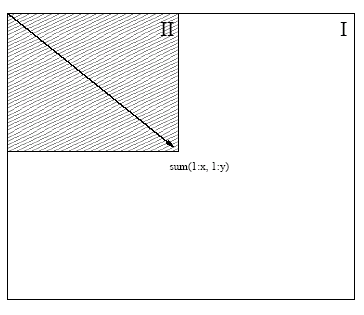
\includegraphics[width=\linewidth]{img/integral_image}
		\caption{Visualisation of an integral image sum}
		\label{fig:integralimage}
	\end{subfigure}
	\begin{subfigure}[t]{0.45\linewidth}
	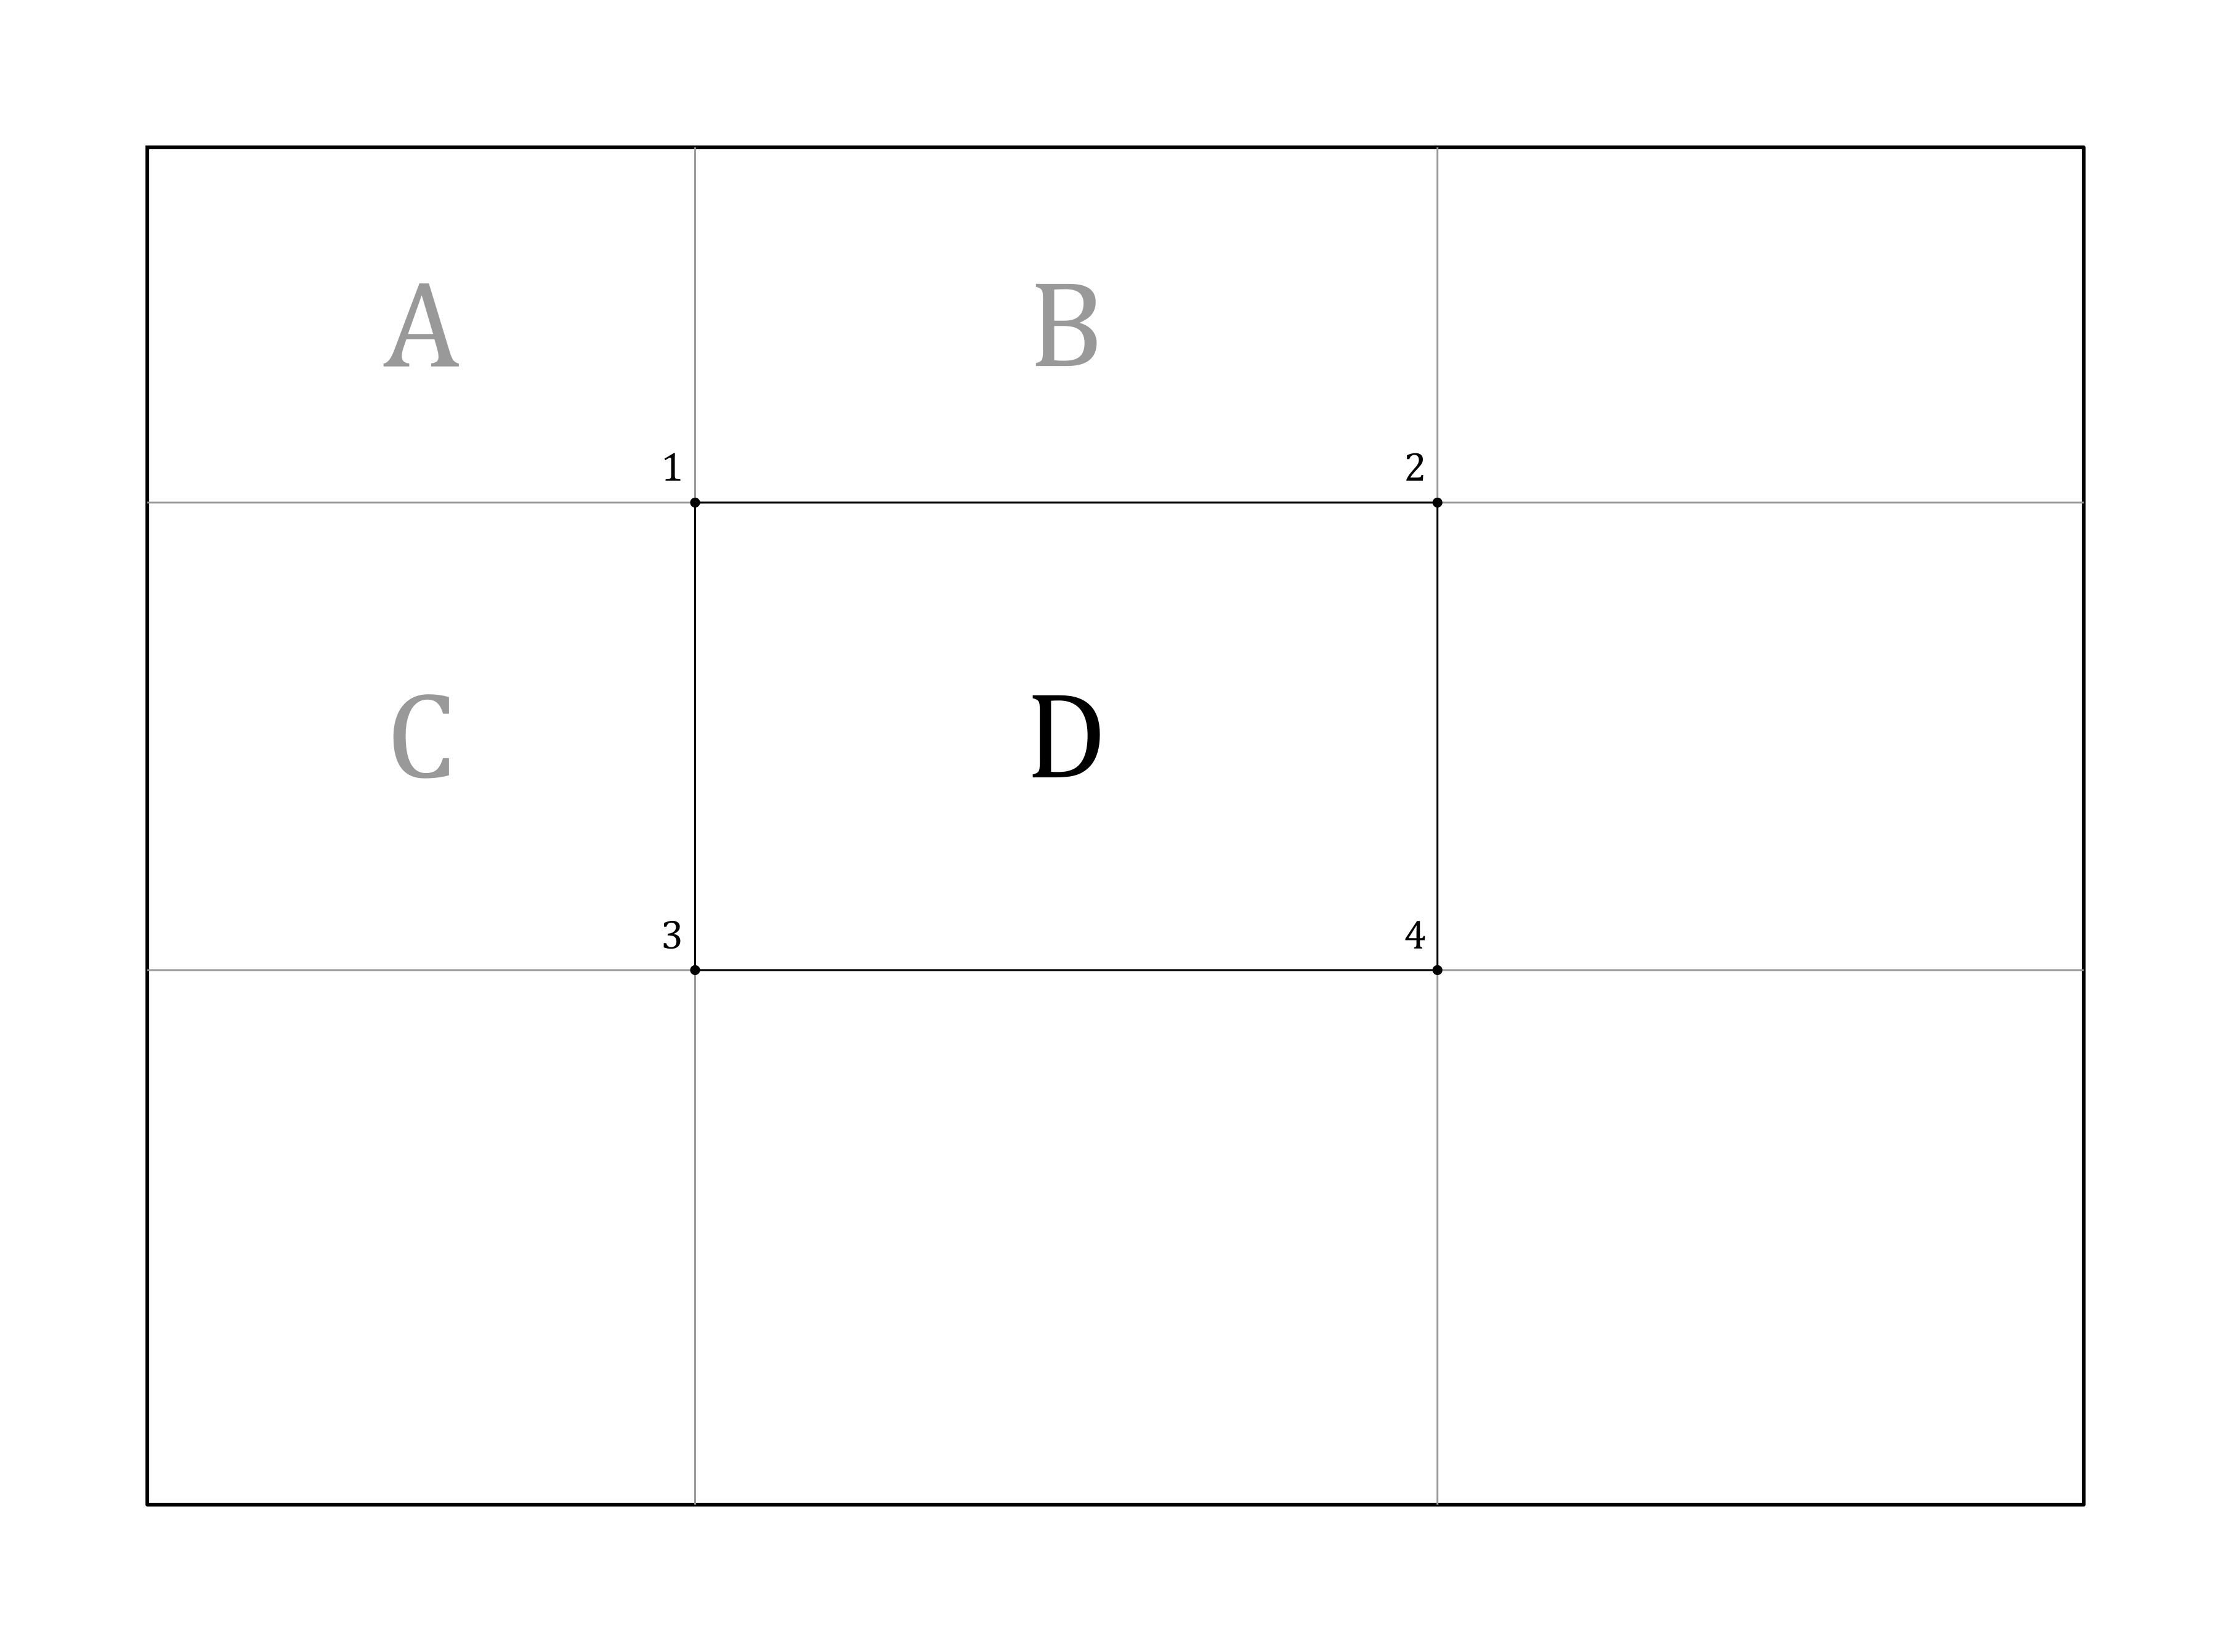
\includegraphics[width=\linewidth]{img/integral_image_haar}
	\caption{Calculating Haar features using an integral image}
	\label{fig:integralimagehaar}
	\end{subfigure}
\end{figure}
The humongous size of the features per sub window can be evaluated by treating each feature as a weak classifier and training important features using adaboost.

\subsection{Face Detection}
The problem is that there are thousands of possible position or scale combinations in the image which need to be evaluated, while true faces are rare in the image.
The idea is thus to dismiss the regions without a face efficiently.
The goal for a classifier is to have a high \emph{true} positive rate (85\%-95\%) and a low \emph{false} positive rate ($10^{-5}-10^{-6}$).
Use this classifier in a cascade which multiplies false and true positive rates. False results are rejected early in the processing.
\begin{center}
	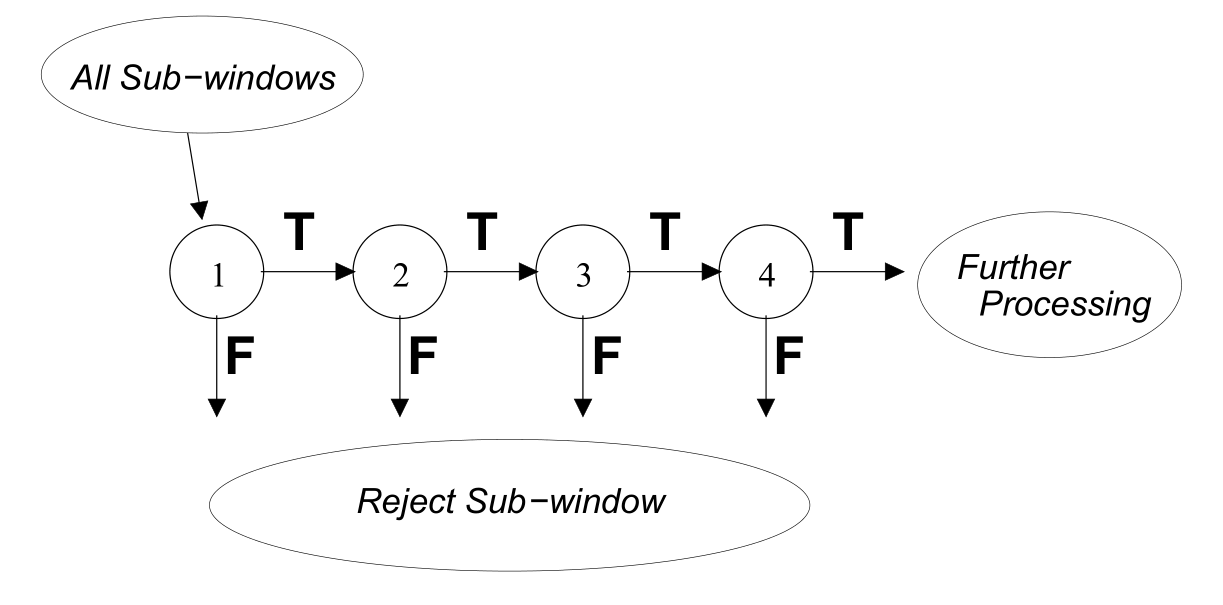
\includegraphics[width=0.6\linewidth]{img/cascade_classifier_approach}
\end{center}

\subsection{HOG for Human Detection}
Detection Pipeline
\begin{itemize}[label=-]
	\item Calculate HOG Descriptors
	\item Collect HOGs in Detection Window
	\item Use Linear SVM for Person or Non-Person Classification
\end{itemize}
\begin{center}
	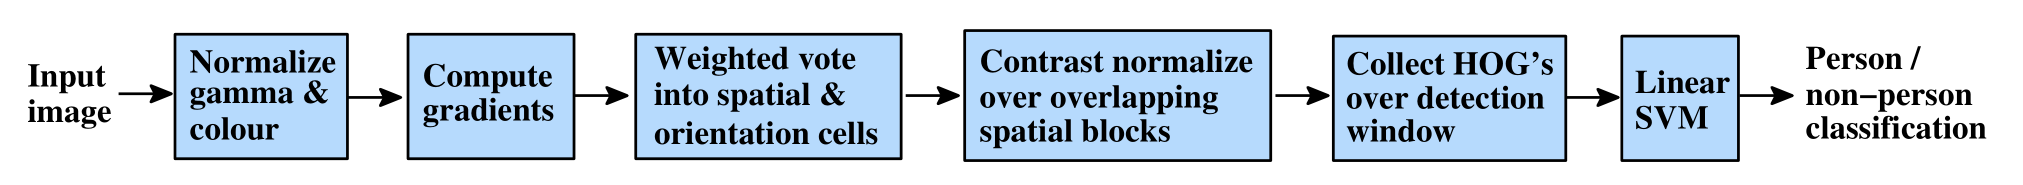
\includegraphics[width=0.8\linewidth]{img/hog_human_detection}
\end{center}

\subsection{OverFeat}
Combine Classification, Localisation and Detection.
\begin{itemize}[label=]
	\item Classification
	\begin{itemize}[label=-,nosep]
		\item CNN
		\item Sliding Windows, apply at every possible pixel and at multiple scales
		\item Subsampling factor of 12
	\end{itemize}
	\item Localisation
	\begin{itemize}[label=-,nosep]
		\item Generate Bounding Box Prediction, as a Regression Problem
		\item Uses the same first five layers in the CNN
	\end{itemize}
	\item Detection
	\begin{itemize}[label=-,nosep]
		\item Combine Classification and Localisation
		\item Merge and accumulate bounding boxes
	\end{itemize}
\end{itemize}

\begin{figure}[tbh]
	\centering
	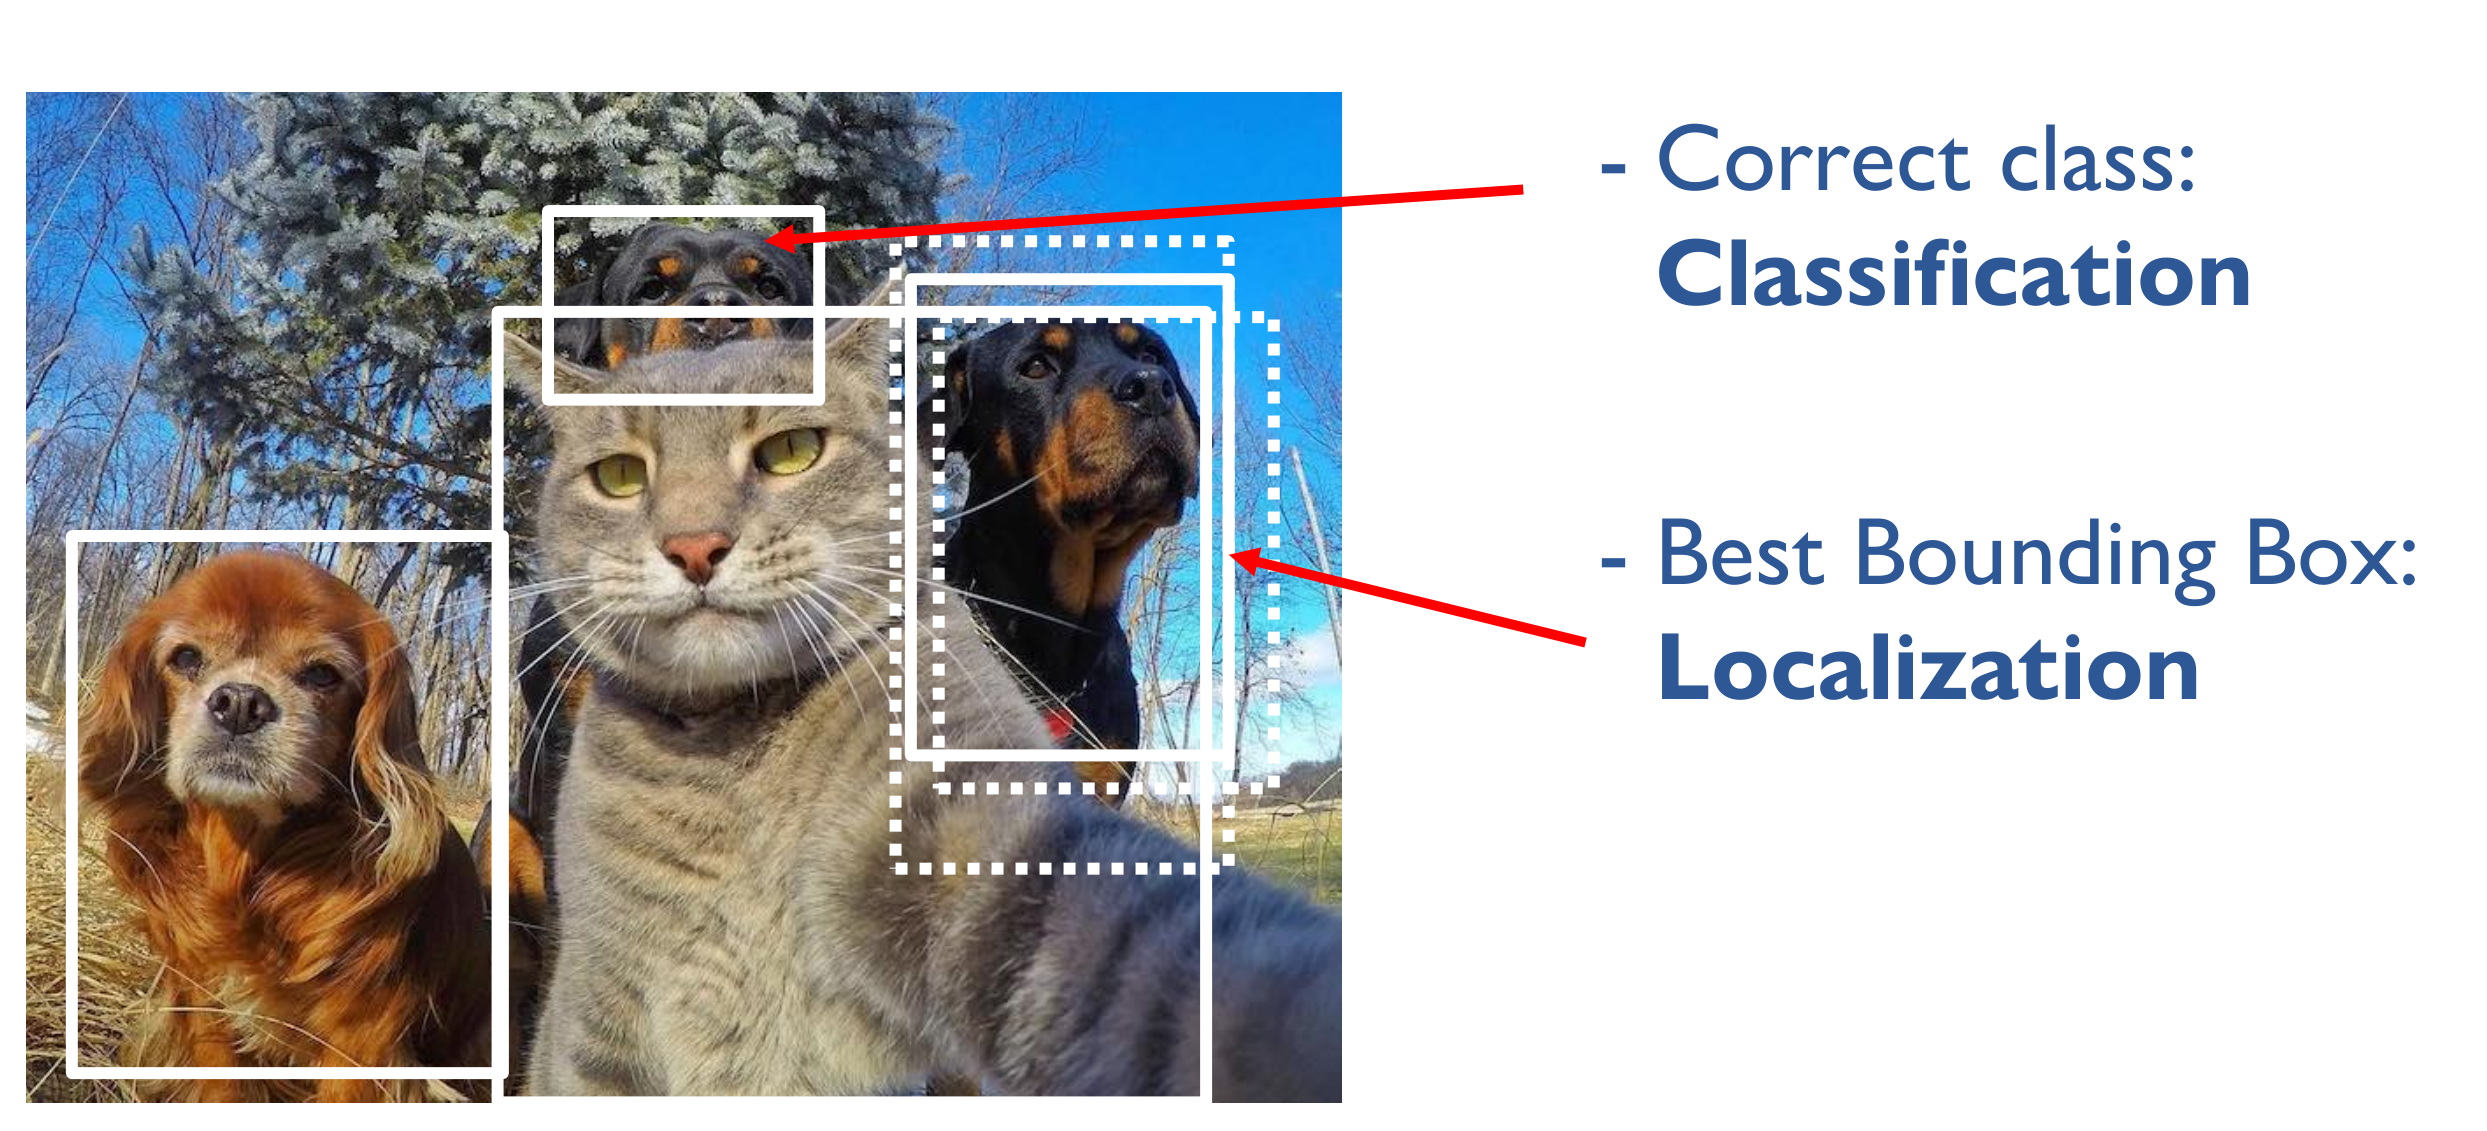
\includegraphics[width=0.7\linewidth]{img/classification_localisation}
	\caption{Classification and Localisation visualised}
	\label{fig:classificationlocalisation}
\end{figure}

Sliding windows have the drawback of the huge numbers of different positions and sizes that need to be evaluated.
A better idea would be to find image regions that are likely to contain an object, which are called region proposals.

\subsection{R-CNN}
Extract region proposals, compute CNN features on these, classify the regions using SVM.
\begin{center}
	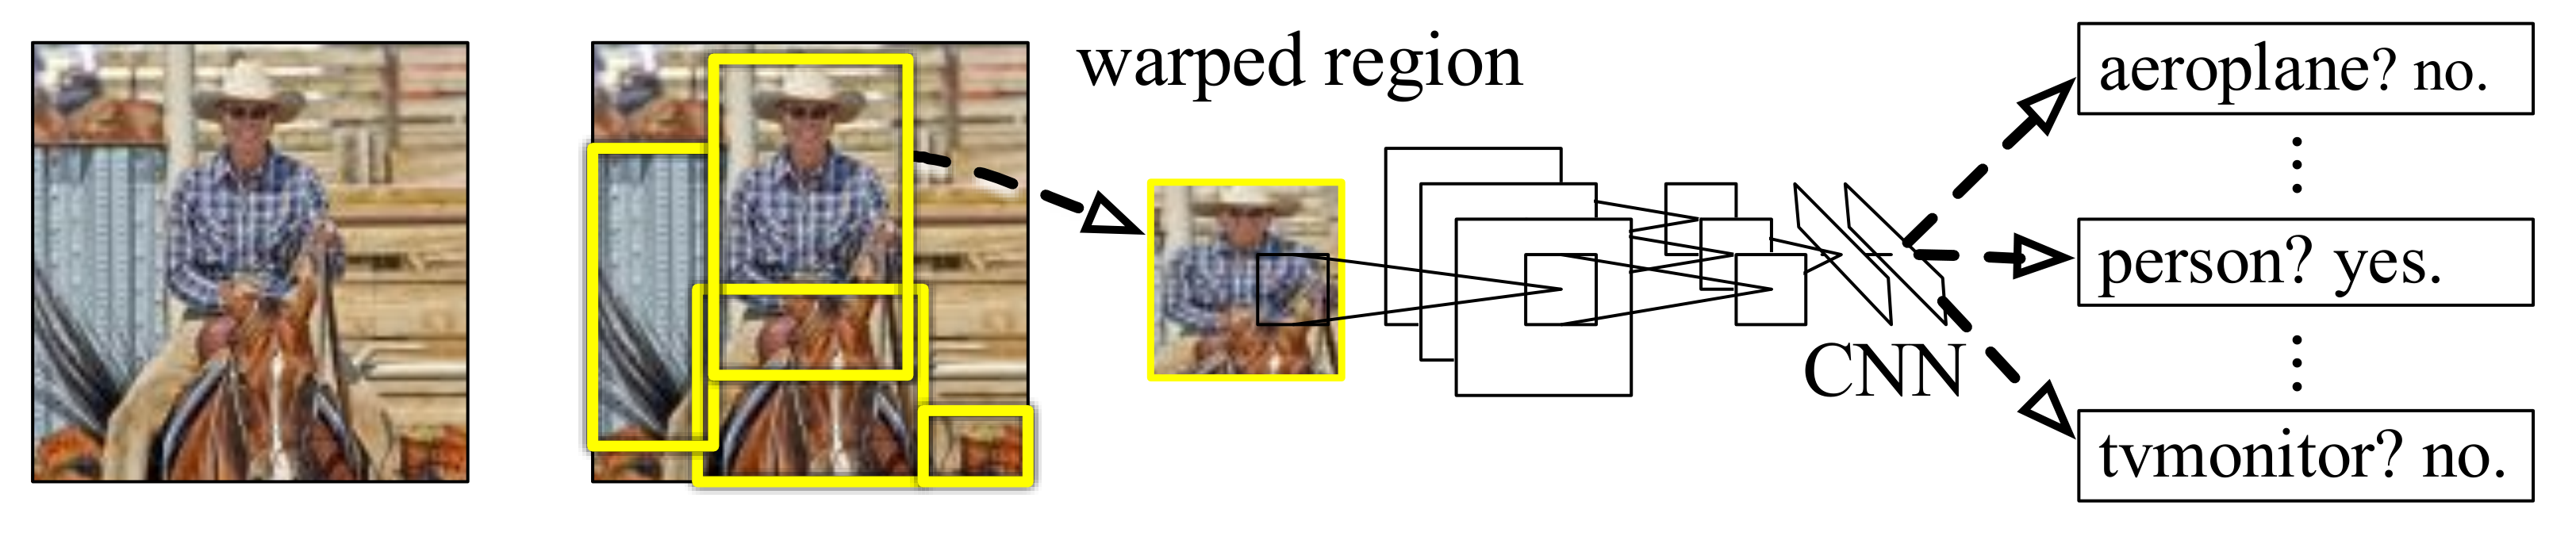
\includegraphics[width=0.7\linewidth]{img/r-cnn}
\end{center}

\begin{center}
	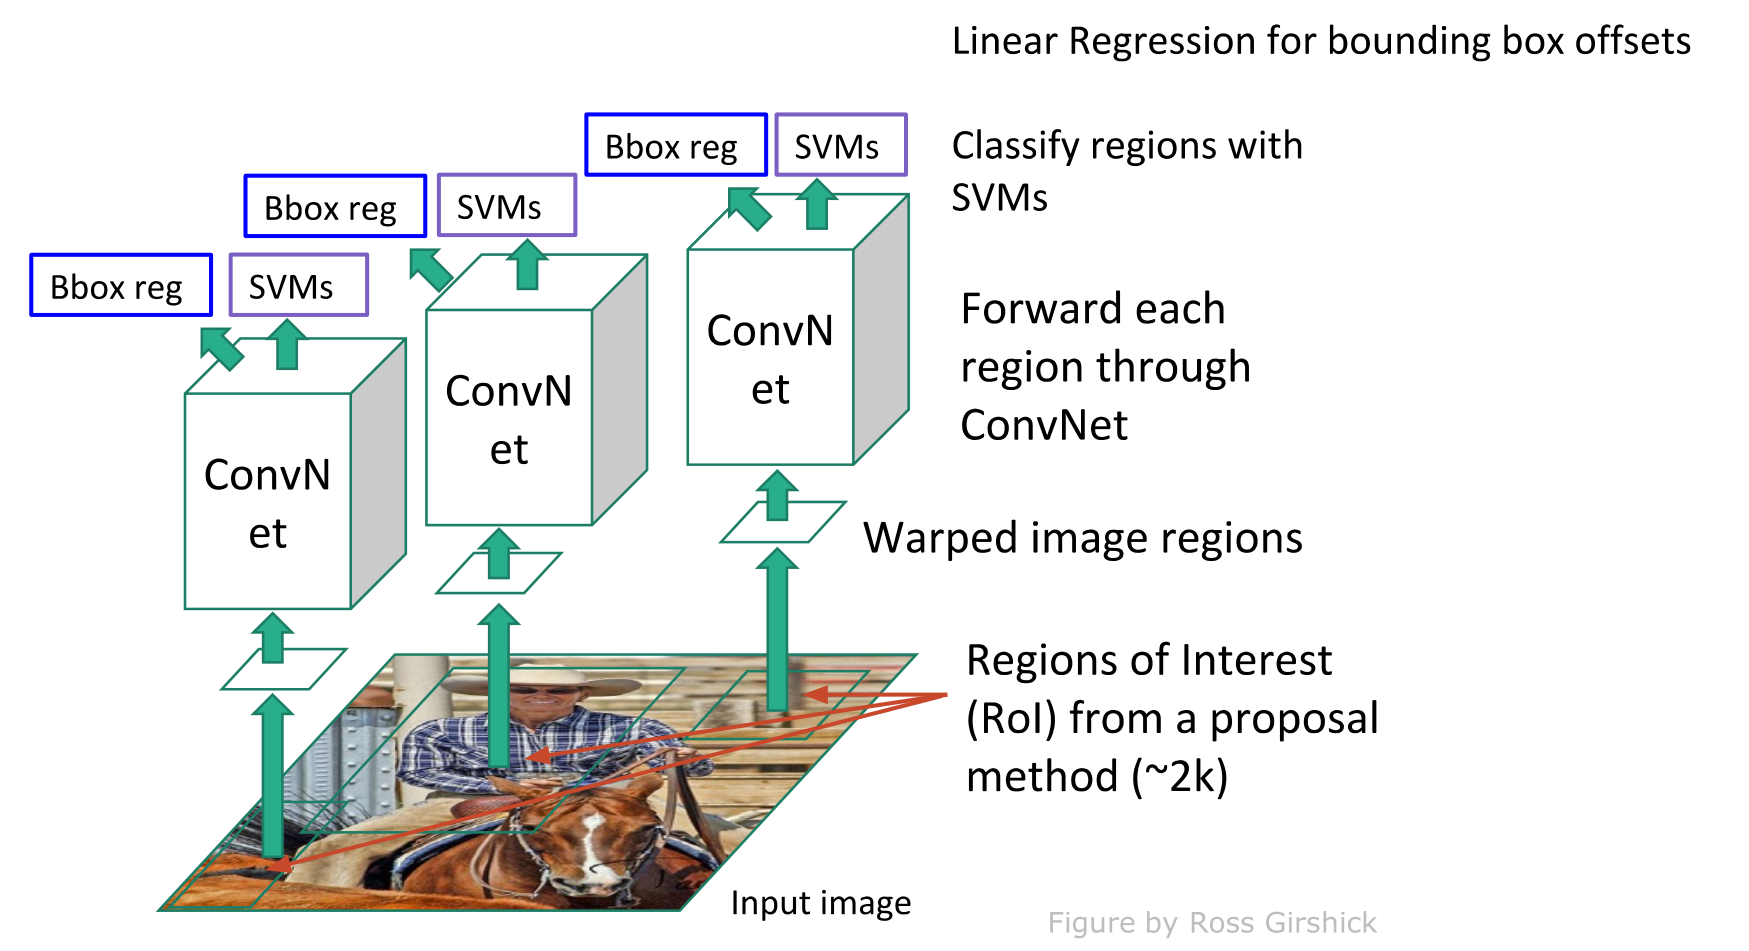
\includegraphics[width=0.7\linewidth]{img/r-cnn_structure}
\end{center}

\subsubsection{Feature Extraction}
\begin{itemize}
	\item Proposal regions are warped to $227\times 227$ pixel images
	\item 4096 Features from $227\times 227$ RGB Image using five Convolutional and two fully connected layers from AlexNet Architecture
	\item Supervised pre-training on the ILSVRC2012 classification data set
	\item Domain-specific fine-tuning is done by continuing training on warped region proposals
\end{itemize}

\subsubsection{Classifier}
Use one linear SVM per class (one true class versus all others), consider regions with overlap of 30\% a positive example and treat the bounding box position as regression problem.

\subsubsection{FAST R-CNN}
Replace SVM of R-CNN with fully connected neural network for classification of objects and refined bounding boxes
\begin{center}
	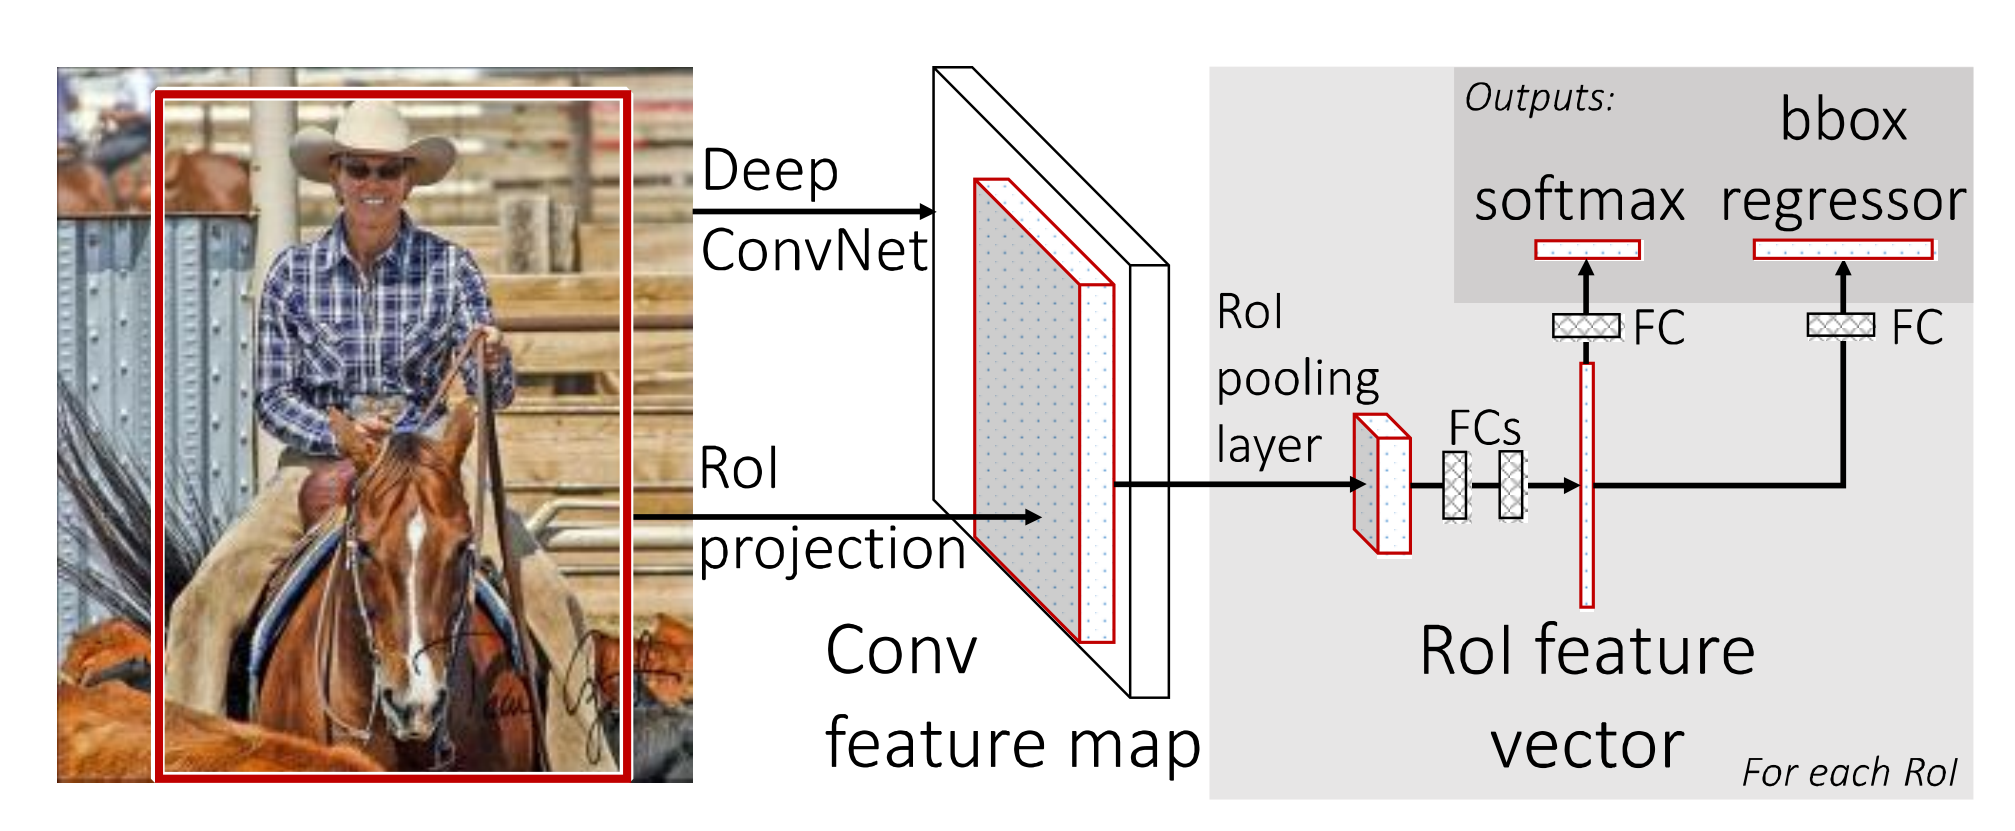
\includegraphics[width=0.7\linewidth]{img/fast_r-cnn_structure}
	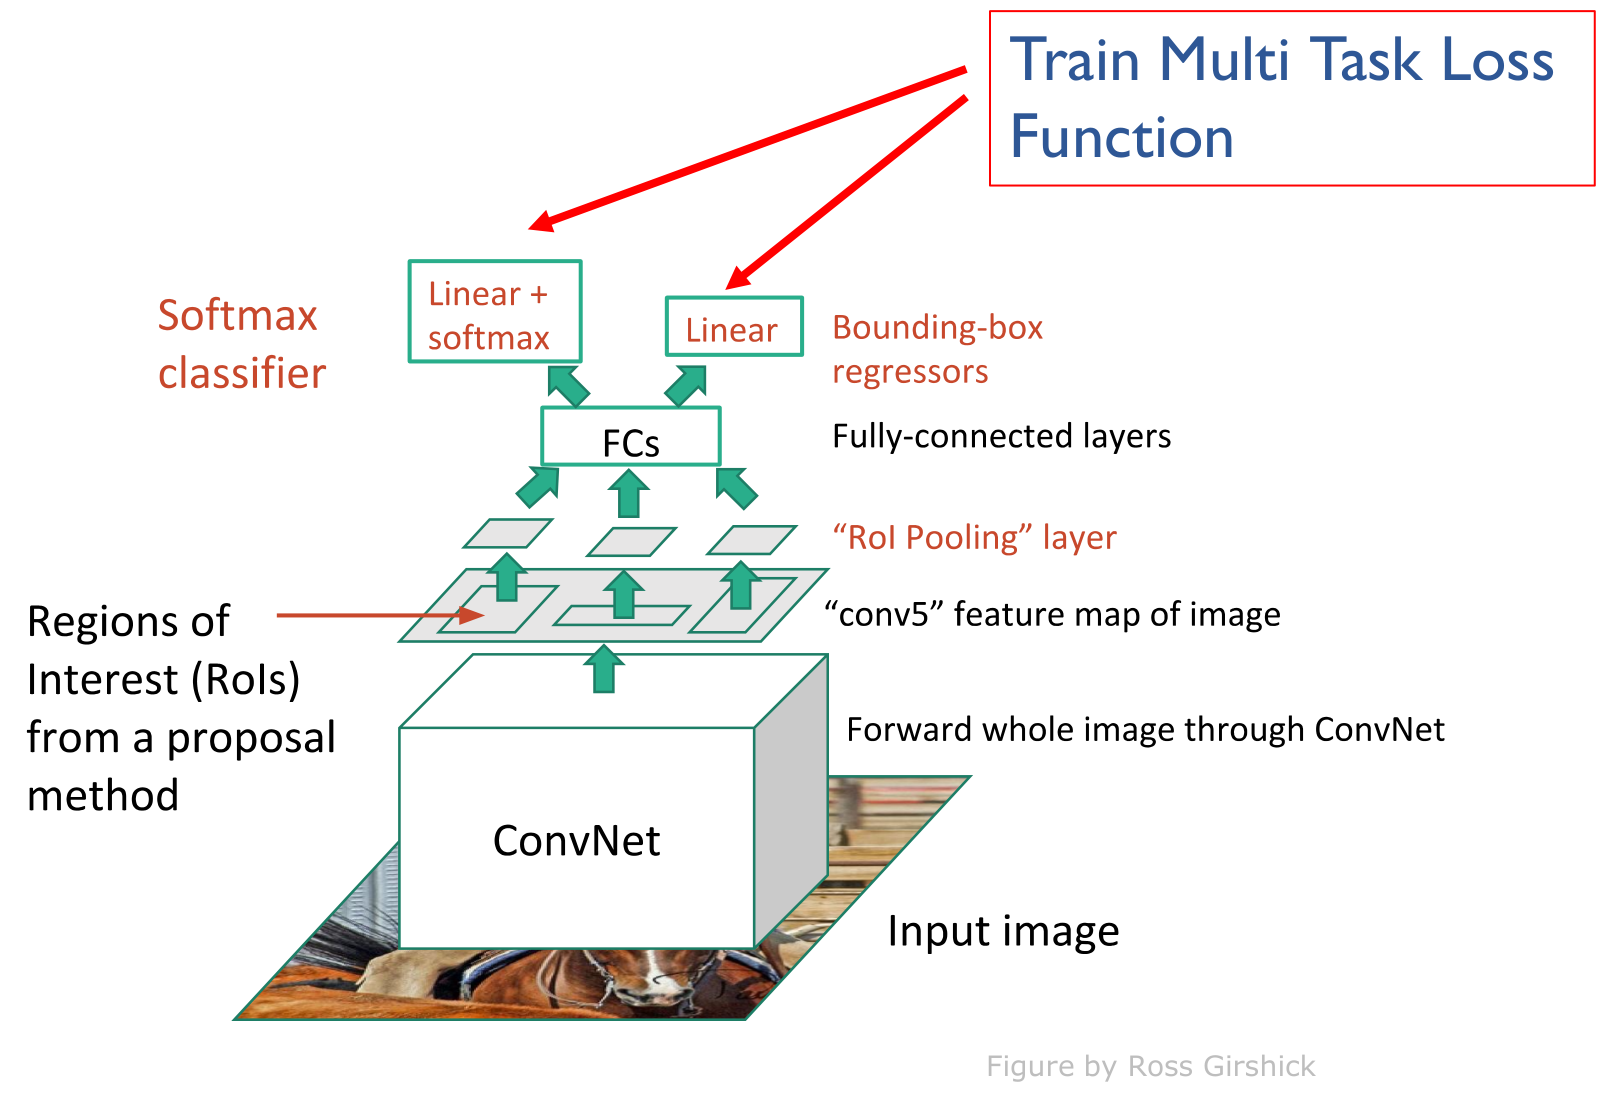
\includegraphics[width=0.7\linewidth]{img/fast_r-cnn_structure2}
\end{center}

\subsection{You Only Look Once (YOLO)}
YOLO is a Single Neural Network that predicts bounding boxes and classification probabilities,
which is very Fast and has good classification but not so good localization properties. The approach is
\begin{itemize}[label=-,nosep]
	\item Divide Image into $S \times S$ grid
	\item Each grid cell predicts B bounding boxes with confidence scores ($x, z, w, h, \text{score}$)
	\item Each grid cell predicts class probabilities (independent of bounding boxes)
	\item Multiply confidence score and probabilities at test time
\end{itemize}

\subsubsection{Improvements}
\begin{itemize}[label=-]
	\item Add Batch Normalisation
	\item Use higher resolution ($448\times 448$)
	\item Use Anchor Bounding Boxes from k-Means Analysis on the training data
	\item Use new base net (darknet19 and darknet 58)
\end{itemize}
